

\textbf{Preventivo orario}

\begin{tblr}{
    colspec={|X[5cm]|X[.5cm]|X[.5cm]|X[.5cm]|X[.5cm]|X[.5cm]|X[.5cm]|X[3.5cm]},
    row{odd}={bg=white},
    row{even}={bg=lightgray},
    row{1}={bg=black, fg=white},
    row{8}={bg=black, fg=white}
}

    Nominativo & Re & Am & An & Pg & Pr & Vf & Ore Totali \\ \hline
    Alberto C. & - & - & - & - & 15 & 2 & 17 \\ \hline
    Bilal El M. & 2 & 3 & - & 4 & - & 2 & 11 \\ \hline
    Alberto M. & 5 & - & 5 & - & - & - & 10 \\ \hline
    Alex S. & - & - & - & 5 & 5 & 5 & 15 \\ \hline
    Iulius S. & - & - & 7 & - & - & 2 & 9 \\ \hline
    Giovanni Z. & - & - & - & - & 10 & - & 10 \\ \hline
    Totale & 7 & 3 & 12 & 9 & 30 & 11 & 72 \\ \hline

\end{tblr}

\textbf{Preventivo economico}

\begin{tblr}{
colspec={|X[5cm]|X[3.5cm]|X[1.5cm]|X[3.5cm]},
row{odd}={bg=white},
row{even}={bg=lightgray},
row{1}={bg=black, fg=white},
row{8}={bg=black, fg=white}
}

Ruolo & Costo orario (€/h) & N. Ore & Costo totale (€) \\ \hline
Responsabile & 30,00 & 7 & 210,00 \\ \hline
Amministratore & 20,00 & 3 & 60,00 \\ \hline
Analista & 25,00 & 12 & 300,00 \\ \hline
Progettista & 25,00 & 9 & 225,00 \\ \hline
Programmatore & 15,00 & 30 & 450,00 \\ \hline
Verificatore & 15,00 & 11 & 165,00 \\ \hline
Totale & \SetCell[c=1]{c} & 72 & 1.415,00 \\ \hline

\end{tblr}

\textbf{Attività svolte}

\paragraph{} Le attività svolte dal gruppo nel secondo periodo sono state:
\begin{itemize}
    \item Analisi dei rischi che possono verificarsi durante lo svolgimento dei processi che compongono il progetto, e delle relative possibili strategie di mitigazione;
    \item In seguito all'individuazione delle tecnologie, progettazione e codifica del PoC;
    \item Colloquio con il prof. Cardin per ottenere delucidazioni riguardo lo studio dei requisiti funzionali;
    \item Prima stesura dei requisiti funzionali del prodotto da sviluppare;
    \item Prosieguo della stesura delle Norme di Progetto;
    \item Studio delle metriche da adottare al fine di misurare la qualità di prodotto e dei processi (particolare attenzione spesa per quest'ultimi);
    \item Webinar$^{G}$ organizzato dall'azienda proponente sull'utilizzo di Docker$^{G}$.
\end{itemize}


\begin{figure}[H] 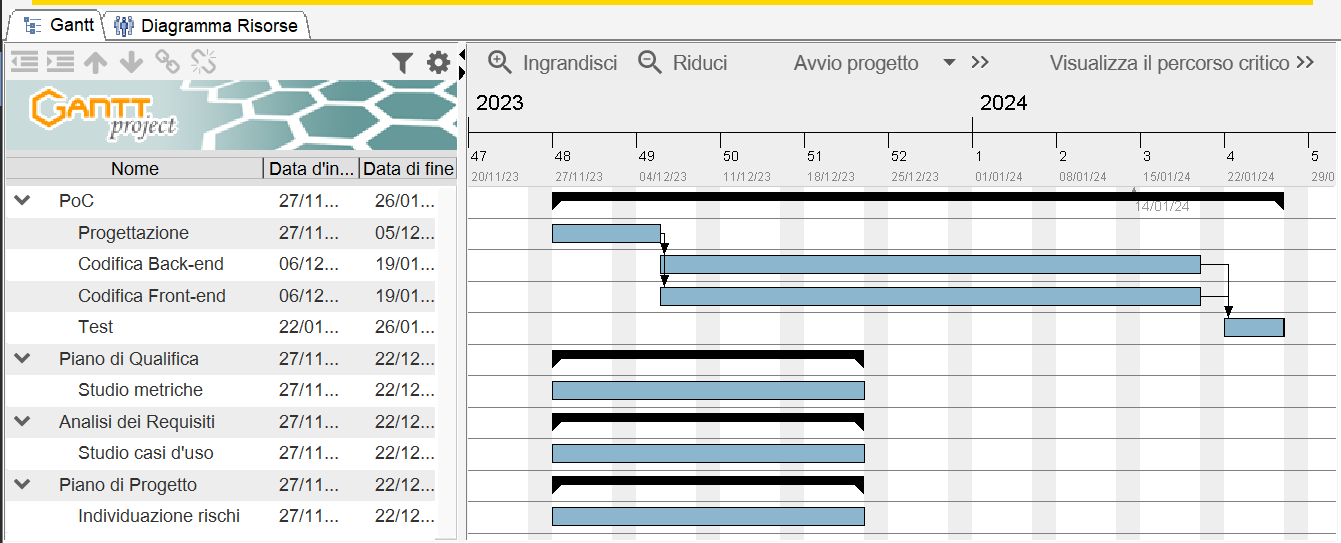
\includegraphics[scale=.6]{GanttSecondoPeriodo.png} \end{figure}

\textbf{Consuntivo orario}

\begin{tblr}{
    colspec={|X[5cm]|X[.5cm]|X[.5cm]|X[.5cm]|X[.5cm]|X[.5cm]|X[.5cm]|X[3.5cm]},
    row{odd}={bg=white},
    row{even}={bg=lightgray},
    row{1}={bg=black, fg=white},
    row{8}={bg=black, fg=white}
}

    Nominativo & Re & Am & An & Pg & Pr & Vf & Ore Totali \\ \hline
    Alberto C. & - & - & - & - & 20 & 5 & 25 \\ \hline
    Bilal El M. & - & - & - & 4 & - & 2 & 6 \\ \hline
    Alberto M. & 2 & 3 & 5 & - & - & - & 10 \\ \hline
    Alex S. & - & - & - & 5 & 5 & 5 & 15 \\ \hline
    Iulius S. & - & - & 3 & 4 & - & 2 & 9 \\ \hline
    Giovanni Z. & - & - & - & - & 15 & - & 15 \\ \hline
    Totale & 2 & 3 & 8 & 13 & 40 & 14 & 80\\ \hline

\end{tblr}

\textbf{Consuntivo economico}

\begin{tblr}{
colspec={|X[5cm]|X[3.5cm]|X[1.5cm]|X[3.5cm]},
row{odd}={bg=white},
row{even}={bg=lightgray},
row{1}={bg=black, fg=white},
row{8}={bg=black, fg=white}
}

Ruolo & Costo orario (€/h) & N. Ore & Costo totale (€) \\ \hline
Responsabile & 30,00 & 2 & 60,00 \\ \hline
Amministratore & 20,00 & 3 & 60,00 \\ \hline
Analista & 25,00 & 8 & 200,00 \\ \hline
Progettista & 25,00 & 13 & 325,00 \\ \hline
Programmatore & 15,00 & 40 & 450,00 \\ \hline
Verificatore & 15,00 & 14 & 165,00 \\ \hline
Totale & \SetCell[c=1]{c} & 80 & 1.260,00 \\ \hline

\end{tblr}

\textbf{Gestione dei ruoli}

\paragraph{}
Nel secondo periodo, il ruolo per il quale è stata spesa la fetta più consistente di ore (50\%),
è stato quello di Programmatore, data la volontà del gruppo di completare entro la fine del periodo
la codifica del PoC e la relativa fase di test (alla quale è stato dedicato il 17\% delle ore). \\
Il 16\% delle risorse è stato dedicato alla figura del Progettista per supportare e guidare i Programmatori nel lavoro di codifica; nonostante la necessità
di proseguire con la stesura della documentazione e con l'analisi dei requisiti funzionali, solo il 10\% delle ore è stato
dedicato al ruolo di Analista; il 3\% delle ore è stato dedicato alla figura del Responsabile e il 3\%
dell'Amministratore.

\pagebreak

\paragraph{Gestione dei rischi}

\begin{itemize}
\item \textbf{Rischio verificatosi:} Conflitti decisionali:
\begin{itemize}
\item \textbf{Esito Piano di Contingenza:} Essendosi presentati punti di vista differenti riguardo le tecnologie da includere nello stack, sia per quanto riguarda la parte di Front-end che quella di Back-end, i membri del gruppo hanno avviato una discussione nella quale considerare i pro e i contro delle differenti proposte; si è deciso di affidare la scelta definitiva ai membri con la maggior expertise nell'ambito dei linguaggi di programmazione;
\item \textbf{Impatto:} L'impatto è stato nullo, grazie alla disponibilità e alla maturità dimostrata da tutti i membri del gruppo nell'affrontare un conflitto decisionale e soprattutto nell'accettarne la risoluzione.
\end{itemize}

\item \textbf{Rischio verificatosi:} Tecnologie da usare:
\begin{itemize}
\item \textbf{Esito Piano di Contingenza:} L'azienda proponente ha offerto al gruppo la possibilità di partecipare ad un Webinar su Docker, permettendo così un avanzamento importante nella codifica del PoC e, soprattutto, un allineamento tra tutti i membri della conoscenza della sopracitata tecnologia. L'utilizzo invece della libreria React si è rivelato più complesso del previsto, richiedendo ore supplementari di studio della documentazione relativa da parte dei programmatori;
\item \textbf{Impatto:} Importante è stato l'impatto del rischio legato alle tecnologie utilizzate per la parte Front-End del PoC, avendo richiesto in totale 10 ore in più nel ruolo di Programmatore rispetto a quelle preventivate inizialmente dal gruppo.
\end{itemize}

\item \textbf{Rischio verificatosi:} Calcolo delle tempistiche:
\begin{itemize}
    \item \textbf{Esito Piano di Contingenza:} Precedentemente all'inizio della pausa natalizia, i membri del gruppo hanno preventivato il fatto che sarebbe potuto avvenire un rallentamento dei lavori, in particolare per quanto concerneva la stesura della documentazione ed in misura minore della codifica del PoC; il rallentamento si è però tradotto in un' interruzione quasi totale della stesura stessa e in generale dell'impegno profuso dai membri e della comunicazione fra gli stessi;
    \item \textbf{Impatto:} L'impatto dell'errato calcolo delle tempistiche è stato notevole, non nella misura di un maggior numero di risorse allocate quanto in uno slittamento di 14 giorni delle scadenze fissate precedentemente dal gruppo al termine del primo periodo, entro le quali era stato prefissato terminare le prime versioni rispettivamente, delle Norme di Progetto e dell'Analisi dei Requisiti.
\end{itemize}
\end{itemize}

\paragraph{}
\textbf{Retrospettiva:} 

Nel secondo periodo, il gruppo ha portato avanti diverse attività: Codifica del PoC, prosieguo della stesura della documentazione ed analisi dei requisiti funzionali; nello svolgimento delle ultime due, si sono verificate
le prime criticità importanti che il gruppo ha dovuto affrontare. Innanzitutto, si è manifestata la necessità di implementare un piano di contingenza per la gestione e mitigazione dei rischi; inoltre i membri del gruppo deputati
all'analisi dei requisiti funzionali, hanno realizzato tardivamente il fatto, da una parte di non aver maturato ancora una piena padronanza della sintassi del linguaggio UML e dall'altra, di non aver eseguito fino a quel
momento un'analisi sufficientemente approfondita degli scenari d'uso e di conseguenza dei requisiti stessi; a questa immaturità, si è aggiunta la volontà da parte del gruppo di ultimare
entro la fine del periodo il PoC, riallocando quindi risorse dal ruolo dell'Analista a quello del Progettista. \\
Infine, nonostante fosse stato preventivato, il rallentamento del ritmo di lavoro da parte dei membri
dovuto alla pausa natalizia, si è trasformato in uno stop totale dei lavori stessi, comportando quindi probabilmente un ritardo nella tabella di marcia del gruppo verso il completamento dell'RTB.
\begin{itemize}
\item \textbf{Obbiettivi raggiunti:}
    \begin{itemize}
        \item Termine della codifica della parte di Front-end del PoC;
        \item Termine della codifica della parte di back-end del PoC;
        \item
    \end{itemize}
    \item \textbf{Obiettivi mancati:}
    \begin{itemize}
        \item Completamento della prima versione delle Norme di Progetto;
        \item Stesura della bozza del Piano di Qualifica;
        \item Completamento della prima versione dell'Analisi dei Requisiti.
    \end{itemize}
\end{itemize}